\section{Amortized Cost}

For many data structures, they need to process a long sequence of operations that access and/or modify the data structures. Knowing the time to process each individual operation is important, which we can measure using the worst-case complexity. However, the time for processing the entire sequence is often more important. In this case, we will use amortized analysis to find the amortized complexity. For example, symbol table in a compiler is analyzed using amortized analysis.

\begin{definition}[Worst-Case Sequence Complexity]
    The worst-case sequence complexity $C(m)$ is defined as
    $$
    C(m) = \max \{ T(\sigma) \mid \text{$\sigma$ is a sequence of $m$ operations} \}
    $$
    $C$ is a function of the length of the sequence.
\end{definition}

If there are many possible initial states, we use the notation $T(\sigma, S_0)$ and $C(m,S_0)$ where $S_0$ is an initial state.

To compute $C(m)$:

\begin{itemize}
    \item To get an upper bound on $C(m)$, prove that for every sequence $\sigma$ of $m$ operations, the time to process $\sigma$ from the initial initial state is $\leq f(m)$. Thus, $C(m) \leq f(m)$.
    \item To get a lower bound on $C(m)$, prove that for some sequence of $m$ operations from the initial state, the time to process $\sigma$ is $\geq g(m)$. Thus, $C(m) \geq g(m)$.
\end{itemize}

\begin{definition}[Amortized Cost] \index{amortized cost}
    The amortized cost per operation for a sequence of $n$ operations is the total cost of the operations divided by $n$. Formally,
    $$
    A(m) = \frac{C(m)}{m}
    $$
    for a sequence of $m$ operations.
\end{definition}

As a motivating example, consider if you borrowed \$100k mortgage to buy a house. You need to pay it back over 10 years. Assume interest rate is 10\% per year.

There are two ways to pay the mortgage:

\begin{enumerate}
    \item Pay \$10k of the principal each year plus interest that has accumulated over the year. For example, if the interest rate is 10\%. Then in the first year, we pay \$10k of the principal and $10\% \times \$100$k which is \$20k in total. In the second year, we pay another \$10k of the principal and $10\% \times \$90$k with a total of \$19k, so on and so forth.
    \item Pay the same amount \$16,274 each year. In the first year, most of the payment is the interest. In the tenth year, most of the payment is sthe principal. We say that the mortgage is \textbf{amortized} over 10 years. Amortization refers to the notion of spreading payments over multiple periods. Instead of paying a variable amount every year, we split the total payment into equal amounts each year.
\end{enumerate}

In general, the worst-case sequence complexity is less than or equal to $m$ times the worst-case complexity. This happens if every operation in that sequence is the worst case. It follows that the amortized complexity is always less than or equal to the worst-case complexity.

\subsection{Amortized Analysis of Sorted Linked List}

Consider a sorted linked list. There are sequence of $m$ \proc{Insert} and \proc{Search} operations starting from an empty list. For complexity measure, we will count element comparisons.

$i$th operation takes less than or equal to $i-1$ steps since before the $i$th operation, the list has length $\leq i-1$. So worst-case time for one operation in a sequence of $m$ operations is $m-1$.

For the amortized complexity, consider the sequence $\proc{Insert}(1), \, \proc{Insert}(2),\, \cdots \proc{Insert}(m)$. In this sequence, the $i$th operation performs exactly $i-1$ comparisons and
$$
T(\sigma) = \sum_{i=1}^m (i-1) = \frac{m(m-1)}{2}
$$
Thus the amortized complexity of insertions and searchings in a sorted linked list is at least $T(\sigma)/m = (m-1)/2$.

In this case, the worst-case complexity is a good upper bound for amortized complexity.

\subsection{Increasing Binary Counter}

Consider an array $X$ $[0,\cdots,k-1]$ of bits representing an integer such that
$$
x = \sum_{i=0}^{k-1} X[i]\cdot 2^i.
$$
Initially, $x=0$.

\begin{figure}[htbp]
    \centering
    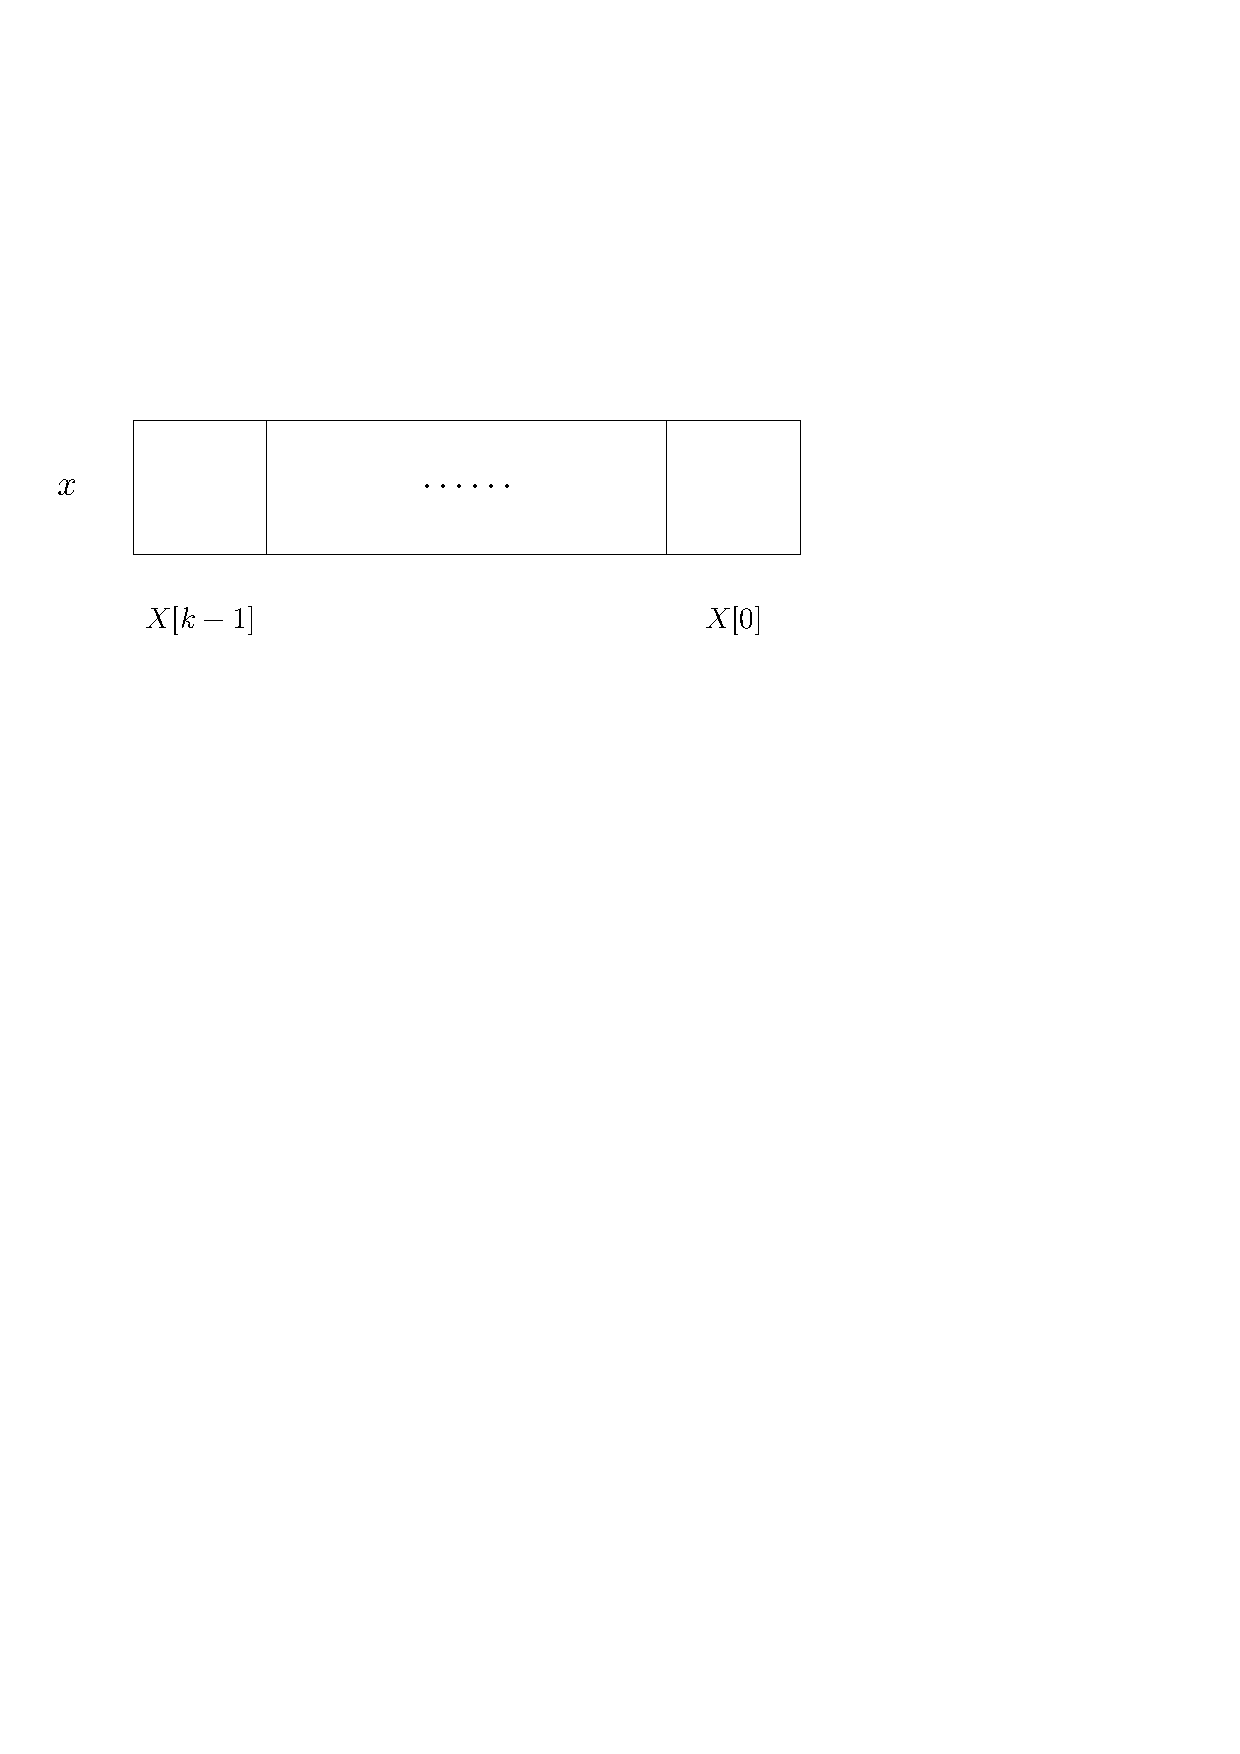
\includegraphics[width=0.4\linewidth]{binary-counter.pdf}
    \caption{The example of a binary counter representing the value $x$ using an array $X$ of length $k$.}
    \label{fig:binary-counter}
\end{figure}

We have an operation $\proc{Increment}(x)$ which adds 1 to $x$ modulo $2^k$.

\begin{codebox}
    \Procname{$\proc{Increment}(X)$}
    \li $i = 0$ 
    \li \While $i<k$ and $X[i] \isequal 1$ \Do
        \li $X[i] = 0$ 
        \li $i = i + 1$ \End
    \li \If $i < k$ \Then
        \li $X[i] = 1$ 
    \End
\end{codebox}

We will count the number of bits flipped as the measure of time complexity. The worst-case number of bit flips in an \proc{Increment} operation is $k$ (e.g. occurs when all bits of $X$ are 1). As an example, consider the sequence of operations to increment a binary counter of 3 bits from 000 to 111.

\begin{figure}[htbp]
    \centering
    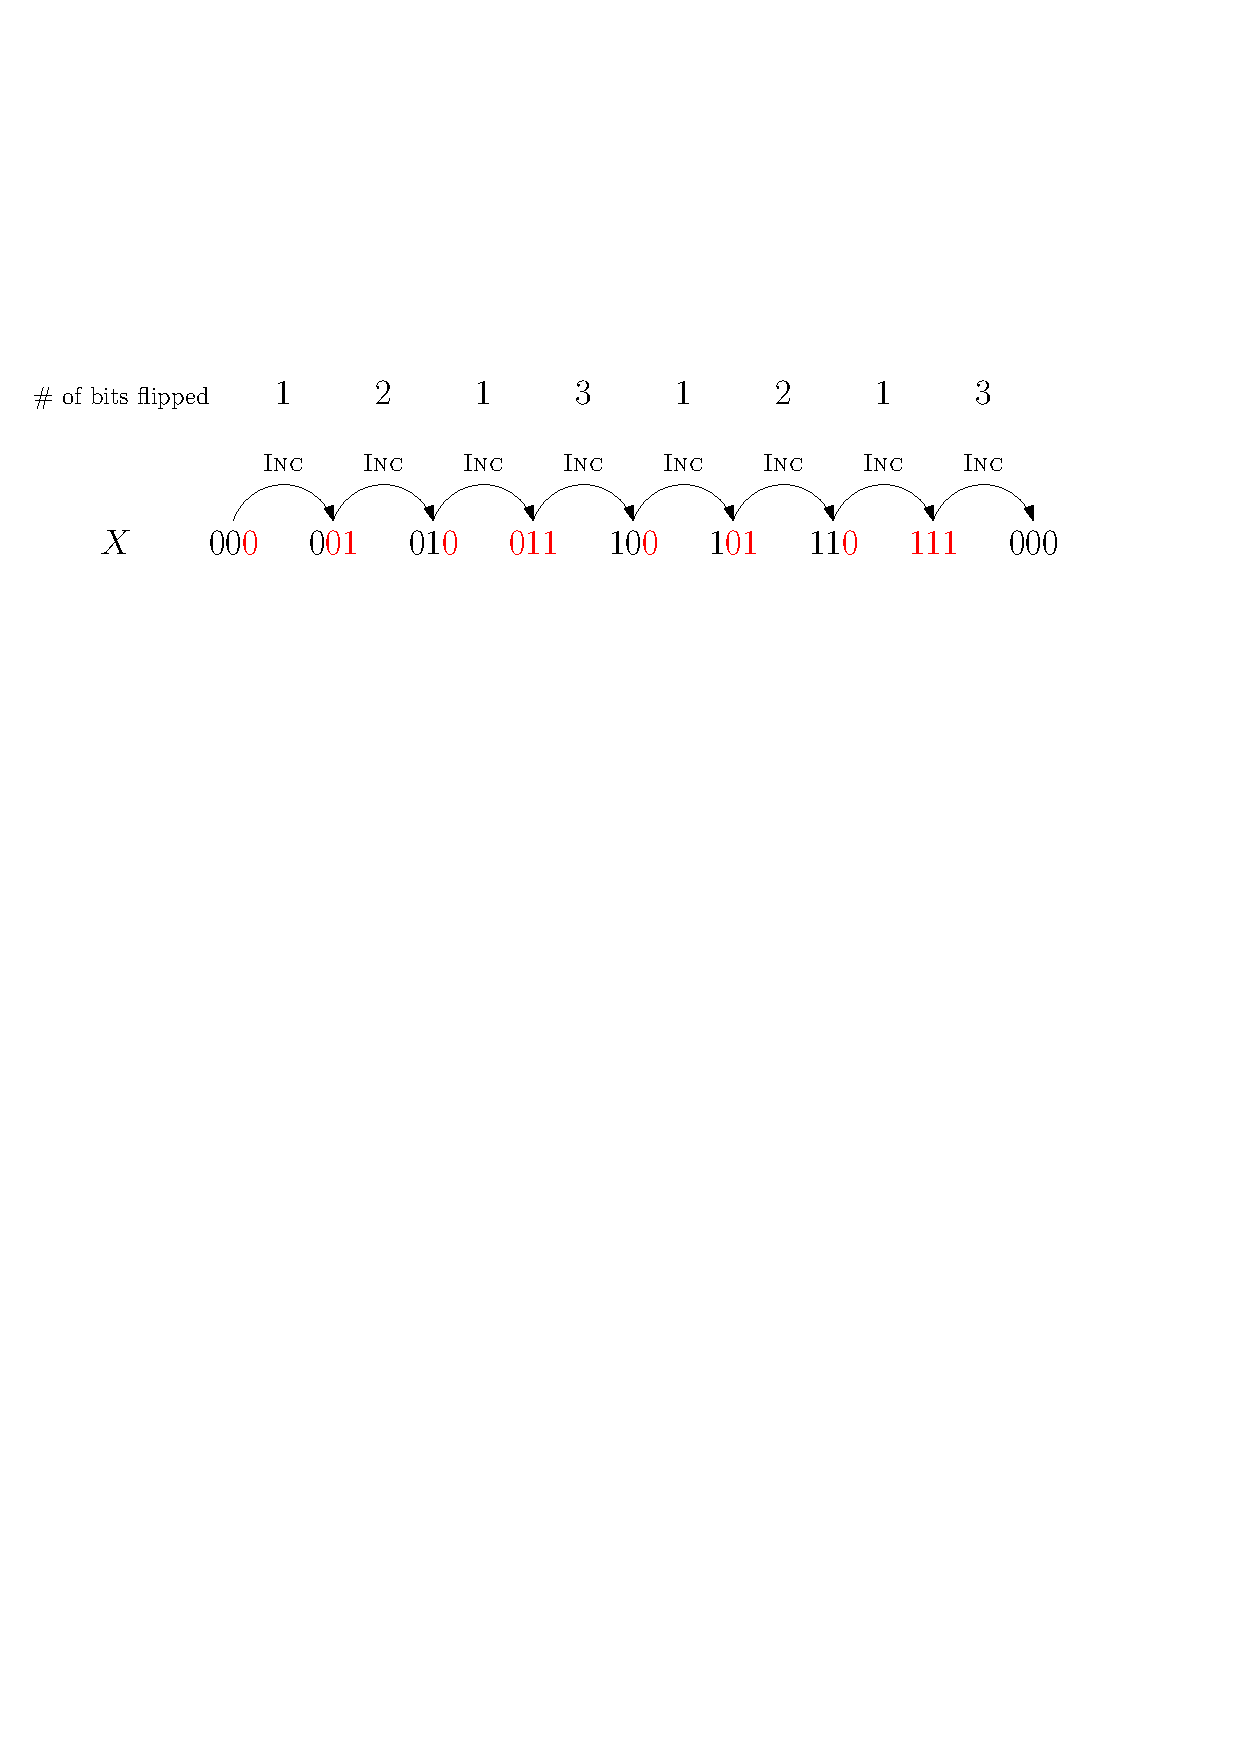
\includegraphics[width=0.8\linewidth]{binary-counter-inc.pdf}
    \caption{The sequence of operations to increment a binary counter of 3 bits from 000 to 111. The bits highlighted in red are the ones to be flipped in the next \proc{Increment} operation.}
    \label{fig:binary-counter-inc}
\end{figure}

There is only one sequence of $m$ \proc{Increment} operations. In this sequence, $X[0]$ is flipped $m$ times; $X[1]$ is flipped $\lfloor m/2 \rfloor$; $X[2]$ is flipped $\lfloor m/4 \rfloor$; and $X[i]$ is flipped $\lfloor m/2^i \rfloor$ times.

Hence, the worst-case sequence complexity is
$$
C(n) = \sum_{i=0}^{k-1} \left\lfloor \frac{m}{2^i} \right\rfloor < m \sum_{i=0}^\infty 2^{-i} = 2m
$$
Thus,
$$
A(m) = \frac{C(m)}{m} \leq 2
$$
while the worst-case complexity of an \proc{Increment} is $k$.

Generally, there are three methods for performing amortized analysis. Although all methods should give us the same answer, depending on the circumstances, some methods will be easier than others.

\begin{itemize}
    \item Aggregate analysis determines the upper bound $T(n)$ on the total cost of a sequence of $n$
    operations, then calculates the amortized cost to be $T(n) / n$.
    \item The accounting method determines the individual cost of each operation, combining its immediate execution time and its influence on the running time of future operations. We use the analogy of a bank account. Prior operations that may impact future operations can store some credits in the bank for uses by future operations. Usually, many short-running operations accumulate credits in small increments, while rare long-running operations use the credits.
    \item The potential method is like the accounting method, but the balance of the imaginary bank account at each state is given by the potential function.
\end{itemize}

\section{Aggregate Method} \index{aggregate method}

Get an upper and lower bound on $C(m)$ worst-case sequence complexity and then divide it by $m$. The previous two analyses on the examples (sorted linked list and binary counter) are all done using the aggregate method.

\section{Accounting Method} \index{accounting method}

In the accounting method, each kind of operation is assigned a fixed charge $a(\id{op})$ called the \textbf{allocated charge} or \textbf{amortized cost} of that operation. \index{allocated charge} \index{amortized cost}

When the allocated cost $a(\id{op})$ is greater than the actual cost of $\id{op}$, the excess is associated with specific objects in the data structure as credit. Credits can be used later to help pay for operations where allocated costs are less than their actual costs. The can be viewed as storing money in a bank account for later uses.

If the total credit in the data structure is always non-negative (i.e. the bank account never runs out of money), then the total actual cost of the sequence of operations is less than or equal to the sum of allocated charges of the operations in the sequence.

To prove that the total credit in the data structure is always non-negative, we will use a credit invariant (similar to loop invariant used to prove correctness). The credit invariant is a rule that says that parts of the data structure with certain properties will have a certain number of credits associated with them. Credit invariants are proved by induction.

Sometimes, credits are needed to establish the credit invariant for the initial state. Then, the total actual cost of the sequence $\leq$ the cost to establish the credit invariant plus the sum of allocated charge to the operations in the sequence.

$$
\begin{aligned}
    \text{total cost of the sequence} \leq & \text{ cost to initially establish the credit invariant } + \\
    & \text{ sum of allocated charges to $m$ operations in the sequence}
\end{aligned}
$$

\begin{remark}
    It is important NOT to explicitly implement the credit system in the code. It is for analysis purpose only.
\end{remark}

We will use the binary counter as a running example when discussing different analysis methods. It is important to define what ``a dollar'' means and what are the allocated charges for each type of operation.

\begin{itemize}
    \item We define that $\$1 = \text{ cost of one bit flip}$.
    \item The initial value of the account is 0. 
    \item The allocated charge to \proc{Increment} is \$2.
\end{itemize}

\textit{Credit Invariant}: Each bit with value value 1 has \$1 credit.

When we flip a bit from 0 to 1, we use \$1 to actually flip that bit, and store the additional \$1 as the credit on that bit (in order to maintain the credit invariant).

When we flip a bit from 1 to 0, the associated \$1 credit at that bit can be used to pay for performing the bit fip.

\begin{proof}
    Initially, all bits are 0, so the credit invariant is vacuously true.

    Assume that the credit invariant is true before an \proc{Increment} operation. Then, all bits of 1 in $X$ contain a \$1 credit.

    Case 1: The $i$ least significant bits $X[0],\cdots,X[i-1]$ are 1, and $X[i] = 0$ for some $i$ such that $0 \leq i \leq k$. The actual number of bit flips in this case is $i+1$. Use the $i$ credits associated with the $i$ least significant bits to pay for flipping these bits from 1 to 0. Use \$1 of allocated charge to pay for flipping $X[i]$ from 0 to 1. Use the remaining \$1 of allocated charge to associate as credit with $X[i]$. All other 1 bits still have \$1 credit. Thus the credit invariant is true after this \proc{Increment} operation.

    Case 2: All of the bits are 1, so all $k$ bits are flippted. Use the $k$ credits on these bits to pay for the flips. This maintains the credit invariant. The \$2 allocated to the current \proc{Increment} are not needed (so they can be donated to charity).

    Then by induction, the credit invariant is true after every \proc{Increment} operation. The cost to establish the credit invariant is 0.

    The total actual cost of $m$ operations $C(m) \leq 0 + 2m$. Hence, the amortized cost $A(m)$ of \proc{Incremente} is at most 2 bit flips.  
\end{proof}

\section{Dynamic Array}

In this section, we will consider the data structure known as dynamic array. It is similar to a regular array, but its length changes according to the ``fullness'' of the array.

\index{dynamic array}

The array will be initialized with a fixed length. Upon calling \textsc{Insert}, it will insert an element into the array, and whenver the current array becomes full, we create a longer array and copy everything into the new array. Similarly, after calling \textsc{Delete}, we will shrink the array whenever the array becomes too empty. If we only consider the worst case, the runtime complexities are bad: $O(n)$ for both operations. However, if we look at the amortized cost, the runtime is actually smaller.

\begin{figure}[htbp]
    \captionsetup{singlelinecheck=false, font=footnotesize, labelsep=space, margin={0pt,1cm}, justification=raggedright}
    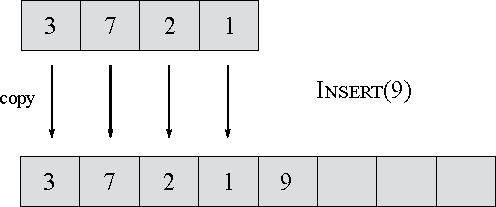
\includegraphics[width=0.4\linewidth]{figures/dynamic_arr_append.pdf}

    \hfill

    \caption[width=0.5\linewidth]{The dynamic array after the operation \textsc{Insert}(9). The length of the new array is doubled, and old elements are copied to the new array.}
\end{figure}

\subsection{Accounting Method Analysis for Dynamic Array}

\begin{figure}[htbp]
    \centering
    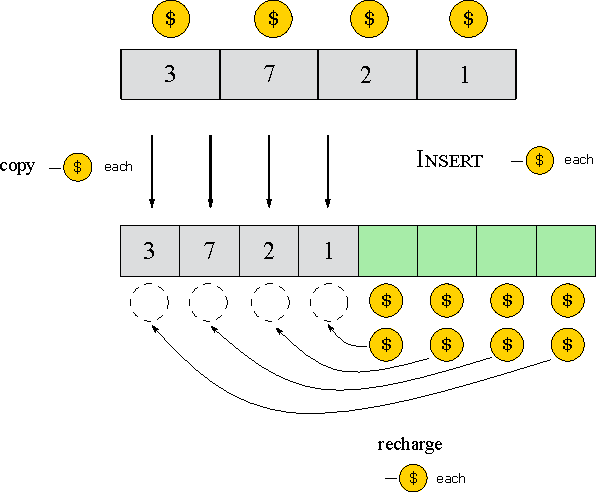
\includegraphics[width=0.6\linewidth]{figures/accounting_method_insert.pdf}
    \caption{<caption>}
\end{figure}

\section{Potential Method}

\vspace{\parskip}

Prepaid wors in represented as potential energy associated with the whole data structure. Potential energy in a data structure can be released to pay for later operations.

\begin{definition}[Potential Function] \index{potential function}
    Let $D$ be some data structure with initial state $D_0$. For each $i = 1,2,\cdots,n$, let $c_i$ be the actual cost of the $i$-th operation and $D_i$ be the resulting data structure after applying the $i$-th operation to data structure $D_{i-1}$.

    The potential function $\Phi$ maps each data structure at state $i$, denoted $D_i$, to a real number $\Phi(D_i)$, which is the potential associated with data structure $D_i$.

    The amortized cost $\hat{c_i}$ of the $i$-th operation with respect to the potential function $\Phi$ is
    $$
    \hat{c_i} = c_i + \Phi(D_i) - \Phi(D_{i-1})
    $$
    And the total amortized cost of $n$ operations is
    $$
    \sum_{i=1}^{n} \hat{c_i} = \sum_{i=1}^{n} \left( c_i + \Phi(D_i) - \Phi(D_{i-1}) \right) = \sum_{i=1}^{n} c_i + \Phi(D_n) - \Phi(D_0)
    $$
\end{definition}

\subsection{Analysis of Binary Counter Using Potential Method}

Let $C_i$ be the configuration after $i$th \proc{Increment}.

Let $\Phi(c)$ be the number of 1 bits in the stored representation of the counter in counfiguration $C$.

$\Phi(C) \geq 0$ for all configurations $C$. $\Phi(C) = 0$ since all bits are 0 initially.